We describe new invariants manifested by the 1d family of Poncelet N-periodics interscribed in the so-called ``homothetic pair'', i.e., a pair of concentric, axis-aligned ellipses with identical aspect ratio. In \cref{fig:confocal_homot} the family is illustrated next to the ``confocal'' family, also known as the {\em elliptic billiard}.

\begin{figure}
    \centering
    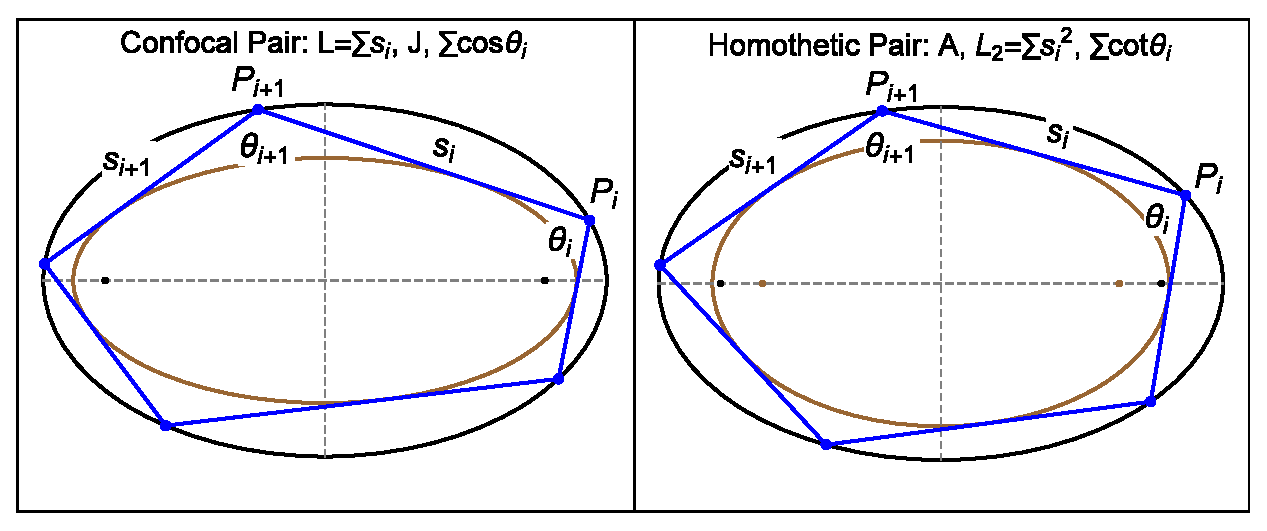
\includegraphics[width=\textwidth]{pics/0010_confocal_homot.eps}
    \caption{\textbf{Left:} A Poncelet 5-periodic in the confocal pair (elliptic billiard). It classically conserves perimeter $L=\sum{s_i}$ and Joachimsthal's constant $J$ \cite{sergei91}. It also conserves $\sum\cos\theta_i$ \cite{akopyan2020-invariants,bialy2020-invariants,reznik2020-intelligencer}. \textbf{Right:} The homothetic family, interscribed between two concentric, axis-aligned, non-confocal, homothetic ellipses. It trivially conserves area $A$. We show it also conserves (i) sum of squared sidelengths $s_i^2$ and (ii) sum of {\em cotangents} of the $\theta_i$.}
    \label{fig:confocal_homot}
\end{figure}

 Two classic elliptic billiard invariants are perimeter $L$ and Joachimsthal's constant $J$  \cite{sergei91}. Recall the latter is tantamount to tangency of sidelines to a confocal caustic. Recently, we've shown this family also conserves the sum of cosines \cite{akopyan2020-invariants,bialy2020-invariants}, as well as product of ``outer'' cosines and certain area ratios \cite{caliz2020-area-product,reznik2020-intelligencer}. For a complete list see \cite{reznik2021-fifty}.

Returning the homothetic family, notice it trivially conserves area $A$ since it is  the affine image of Poncelet polygons between two concentric circles.

\subsection*{Main Results} Using properties of trigonometric polynomials (see \cref{sec:trig-polys}), we show that the homothetic family conserves:

\begin{enumerate}
    \item \cref{lem:norm2}: sum of squared distances from the vertices to any point; see \cref{fig:homot_norm}.
    \item \cref{prop:sqr_si}: the sum of {\em squared} sidelengths.
    \item \cref{th:cot}: the sum of internal angle cotangents.
    \item \cref{prop:dist-focus}: the sum of distances from the vertices to a focus of the external ellipse.
    \item \cref{cor:kappa}: the sum of curvatures $\kappa_i^{-2/3}$ at each vertex.
\end{enumerate}

In the $N=3$ case, a harmonious corollary of the first two results is that the family conserves the Brocard angle $\omega$; see \cref{fig:brocard-n3}. In fact, the idea for the third result is the fact that in a triangle, $\cot\omega=\cot\theta_1+\cot\theta_2+\cot\theta_3$ \cite[Brocard Angle]{mw}. Though for $N>3$ the Brocard angle $\omega$ is no longer defined, magically, the sum of angle cotangents remains invariant.

\begin{figure}
    \centering
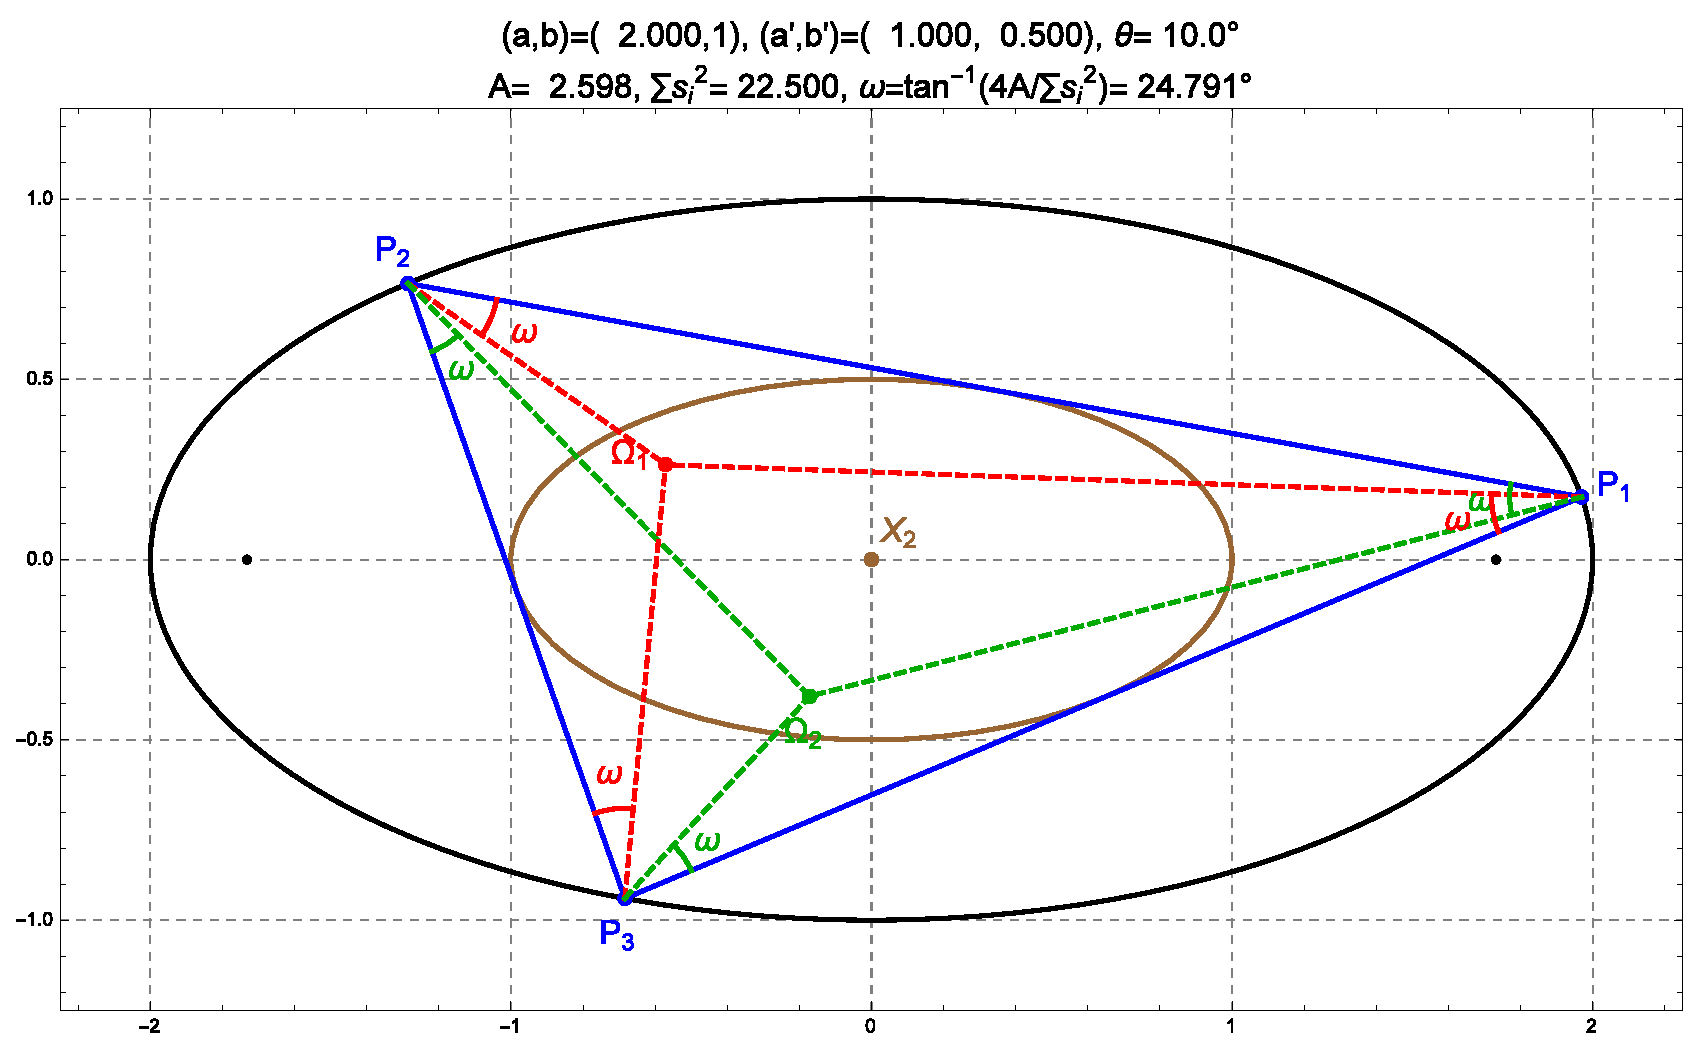
\includegraphics[width=\textwidth]{pics/0040_brocard_n3.eps}
\caption{The family of 3-periodics in the homothetic pair conserve area, sum of squared sidelengths and the Brocard angle $\omega$ which is the particular angle of rotation of sidelengths such that they concur at the two Brocard points $\Omega_1$ and $\Omega_2$. $X_2$ is barycenter which remains stationary over the family at the common center. \href{https://youtu.be/2fvGd8wioZY}{Video 1} and \href{https://youtu.be/13i3JGY-fK4}{Video 2}.}
    \label{fig:brocard-n3}
\end{figure}

Below we only describe Poncelet families of simple N-gons. However all claims hold for self-intersected ones as well.

